\documentclass[10pt,conference]{IEEEtran}

% ===================== PACKAGES =====================
\usepackage[utf8]{inputenc}
\usepackage[T1]{fontenc}
\usepackage{amsmath,amssymb,amsfonts,mathtools}
\usepackage{physics}
\usepackage[draft]{graphicx}   % NOTE: draft mode is the SAFE DEFAULT, so the
                                % document still compiles for any figure whose
                                % file is not yet present (e.g. future
                                % double-well figures). Figures that DO have a
                                % real file attached use the per-image
                                % override `draft=false` in their
                                % \includegraphics call, so they render
                                % normally regardless of the package default.
\graphicspath{{../../figures/}{../../figures/HO/}}
\usepackage{booktabs}
\usepackage{array}
\usepackage{url}
\usepackage[hidelinks]{hyperref}

\begin{document}

\title{A Modular Numerical Pipeline for the Quantum-to-Classical\\
Transition of Heat Capacity: DVR-Based Simulation\\
of Smooth 1-D Potentials}

\author{
\IEEEauthorblockN{Nadav Jean}
\IEEEauthorblockA{
\textit{Department of Chemical Engineering}\\
\textit{Technion -- Israel Institute of Technology}\\
Haifa, Israel\\
Course 00540367 -- Research Project 1, Spring 2026 (Semester 6)\\
Supervisor: Dr.\ David Gelbwaser-Klimovsky \quad Student ID: [insert]}
}

\maketitle

\begin{abstract}
The long-term goal of this research line is to identify regimes in which a quantum heat machine can approach the Carnot bound more closely, at finite power, than its classical counterpart -- not by violating the second law, but by exploiting the enhanced energy fluctuations of a quantized spectrum, in the spirit of recent quantum-thermodynamics results \cite{campisifazio2016,ye2017}. Because heat capacity \emph{is} a direct measure of those fluctuations, this project builds the numerical groundwork for that search: a pipeline that computes $C_v(T)$ for the quantum and classical versions of \emph{any} smooth one-dimensional potential, and locates the classical limit through an $\hbar$-scaling parameter $\xi$ \cite{gelbwaser2018}. Energy levels are obtained from a Colbert--Miller sinc discrete variable representation (DVR) \cite{colbertmiller1992,lightcarrington2000}, and the classical limit is located by scanning $\xi$ until $C_v(\xi)$ settles onto a plateau -- a numerical realization of the textbook semiclassical statement that shrinking $\hbar$ packs more levels into a fixed energy window -- while a companion criterion rejects the collapse of $C_v$ that occurs once the finite computed spectrum is exhausted. The solver is validated against the analytically solvable harmonic oscillator (HO) and is now being extended to the anharmonic double well. We discuss the Schottky anomaly as the common signature of \emph{any} hard edge in an otherwise continuous spectrum, whether that edge is a numerical truncation artifact or the genuine, exponentially small tunnelling splitting of a double well \cite{kozin2025} -- the latter being a candidate for the kind of quantum enhancement motivating the project.
\end{abstract}

\begin{IEEEkeywords}
quantum thermodynamics, discrete variable representation, heat capacity, classical limit, Schottky anomaly, quantum heat engines
\end{IEEEkeywords}

% ===================== I. INTRODUCTION =====================
\section{Introduction}
\label{sec:intro}

\subsection{Motivation: Toward More Efficient Quantum Heat Machines}
The broader aim behind this project is to find operating regimes in which a quantum heat machine outperforms its classical counterpart -- not by exceeding the Carnot efficiency, which the second law forbids for any working substance, but by \emph{approaching} that bound more closely while still delivering finite power. An ideal Carnot cycle is reversible only in the limit of infinitely slow operation, where its power output vanishes; any real engine that runs in finite time necessarily falls short of $\eta_C=1-T_c/T_h$, and how far short depends on the thermodynamic properties of the working substance itself. Recent work in quantum thermodynamics has shown that a working substance with strongly enhanced energy fluctuations -- for instance, near a critical point -- can let a heat engine approach the Carnot point without sacrificing power \cite{campisifazio2016}, and that the heat capacity of a small quantum system, including its finite-size corrections, directly sets the work a cyclic engine can extract \cite{ye2017}. Since $C_v(T)=k_B\beta^2\mathrm{Var}(E)$ (Section~\ref{sec:theory}) is by definition a measure of those fluctuations, a potential whose \emph{quantum} heat capacity exceeds its \emph{classical} value over some temperature range -- the Schottky-type enhancement discussed in Section~\ref{sec:schottky} -- is a natural place to look for this effect. Realizing such an enhancement in an actual device is well beyond a single semester and is not attempted here.

This report documents the groundwork for that longer-term search: a general-purpose numerical tool, built and validated this semester, that computes $C_v(T)$ for the quantum system \emph{and} its classical counterpart for any smooth one-dimensional potential, using the $\hbar$-scaling parameter $\xi$ introduced below. Having such a tool available for an arbitrary potential -- rather than only the textbook cases with closed-form spectra -- is the necessary first step before the question of where, and by how much, quantum $C_v$ exceeds classical $C_v$ can be explored systematically.

\subsection{The $\hbar$-Scaling Method}
The classical limit is reached formally by $\hbar \to 0$. Since $\hbar$ is a fixed constant, the project instead scans a dimensionless factor $\xi$ that plays the role of $1/\hbar$: scaling both temperature and potential energy by $\xi^2$ is mathematically equivalent to sending $\hbar \to \hbar/\xi$ \cite{gelbwaser2018}. As shown in Section~\ref{sec:theory}, this is the same limit the semiclassical approximation takes when it replaces a discrete spectrum with a smooth density of states, which is what justifies using the $\xi$-plateau as a numerical stand-in for $\hbar\to0$.

The remainder of this report is organized as follows. Section~\ref{sec:theory} develops the theoretical and semiclassical background, together with the analytical harmonic-oscillator and box-potential benchmarks derived earlier in the project. Section~\ref{sec:dvr} outlines the physical reasoning behind the DVR method and its automatic grid configuration. Section~\ref{sec:arch} summarizes the computational workflow. Section~\ref{sec:xiconv} discusses the classical-limit search. Section~\ref{sec:systems} presents the systems studied this semester, with the harmonic-oscillator validation figures produced so far. Section~\ref{sec:schottky} discusses the Schottky anomaly and its two roles in this project. Section~\ref{sec:results} reports validation results, Section~\ref{sec:history} summarizes the main numerical refinements made this semester, and Section~\ref{sec:future} outlines planned work for the summer continuation.

% ===================== II. THEORY =====================
\section{Theoretical Background}
\label{sec:theory}

\subsection{Heat Capacity from the Canonical Partition Function}
For a system with discrete energy levels $\{E_n\}$ at inverse temperature $\beta = 1/(k_B T)$, the partition function is $Z = \sum_n e^{-\beta E_n}$, and the heat capacity follows from the variance of the energy,
\begin{equation}
C_v(T) = k_B \beta^2 \left[\expval{E^2} - \expval{E}^2\right] = k_B\beta^2\,\mathrm{Var}(E).
\label{eq:cv_general}
\end{equation}
Physically, Eq.~\eqref{eq:cv_general} says that heat capacity \emph{is} a measure of thermal energy fluctuations: a system whose accessible states span a wide range of energies at temperature $T$ absorbs heat easily (large $C_v$), while a system frozen into one or two states cannot fluctuate and $C_v\to0$. This single relation is used throughout, whether $\{E_n\}$ comes from a closed-form expression or from a numerical diagonalization -- the physics does not care how the spectrum was obtained.

\subsection{The $\hbar$-Scaling Route to the Classical Limit}
Following \cite{gelbwaser2018} (Eq.~S7 therein), the energy levels of a potential scaled by $\xi^2$ obey
\begin{equation}
\frac{E_n\!\left(\hbar_{\text{eff}}=\hbar,\ \xi^2 V(x)\right)}{\xi^2} = E_n\!\left(\hbar_{\text{eff}}=\frac{\hbar}{\xi},\ V(x)\right).
\label{eq:scaling}
\end{equation}
For systems without a closed-form $E_n(\hbar_{\text{eff}})$, Eq.~\eqref{eq:scaling} is realized by scaling \emph{both} temperature and potential by $\xi^2$, i.e. evaluating Eq.~\eqref{eq:cv_general} with $E_n \to E_n/\xi^2$.

\subsubsection{Valid window for $\xi$}
Any numerical spectrum is truncated at a finite highest computed level $E_{\max}$, so the plateau in $C_v(\xi)$ can only be trusted inside a finite window. For the level spacing to be negligible on the scale of $k_BT$ -- the condition for the sum over states to look like the continuous classical integral -- the semiclassical continuum condition requires
\begin{equation}
\xi \gg \sqrt{\beta\,\Delta E}.
\label{eq:xilower}
\end{equation}
At the same time, the truncated sum must not be distorted by the artificial edge at $E_{\max}$: that highest level must remain thermally inaccessible,
\begin{equation}
\xi \ll \sqrt{\beta\,E_{\max}}.
\label{eq:xiupper}
\end{equation}
Combining Eqs.~\eqref{eq:xilower}--\eqref{eq:xiupper} gives the plateau window actually searched numerically,
\begin{equation}
\sqrt{\beta\,\Delta E} \;\ll\; \xi \;\ll\; \sqrt{\beta\,E_{\max}}.
\label{eq:xiwindow}
\end{equation}
The lower bound is the semiclassical continuum condition introduced above; the upper bound is a purely numerical artifact of working with a finite basis (Section~\ref{sec:schottky} returns to this distinction).

\subsection{Analytical Benchmarks}
Two systems with closed-form solutions anchor the numerical pipeline and illustrate the correspondence principle explicitly.

\subsubsection{Harmonic oscillator (HO)}
With $E_n = \hbar\omega(n+\tfrac12)$, the partition function is a geometric series, $Z^{\text{HO}} = e^{-\beta\hbar\omega/2}/(1-e^{-\beta\hbar\omega})$, giving the Einstein oscillator heat capacity
\begin{equation}
C_v^{\text{HO}} = \frac{1}{4}k_B\left[\beta\hbar\omega\,\operatorname{csch}\!\left(\frac{\beta\hbar\omega}{2}\right)\right]^2 .
\label{eq:cvho}
\end{equation}
Taking $\xi\to\infty$ in the scaled version of Eq.~\eqref{eq:cvho} (via L'H\^opital's rule) gives $C_v^{\text{HO,classical}} = k_B$: exactly the equipartition value expected from the two quadratic (kinetic + potential) degrees of freedom in the HO Hamiltonian. Physically, $\beta\hbar\omega\to0$ is the statement that the thermal energy $k_BT$ vastly exceeds the level spacing $\hbar\omega$, so the discreteness of the ladder becomes invisible -- the same conclusion as Eq.~\eqref{eq:xilower} with $\Delta E=\hbar\omega$.

\subsubsection{Box potential}
With $E_n = n^2 E_g$ and no closed-form sum, Eq.~\eqref{eq:cv_general} is evaluated by truncating the infinite series; equipartition (one quadratic, kinetic-only, degree of freedom) predicts $C_v^{\text{box,classical}} = \tfrac12 k_B$. This system was used early in the project to validate the variance-based formula and the truncated-sum approach before moving to potentials with no closed form at all.

% ===================== III. DVR METHOD =====================
\section{Physical Basis of the Numerical Method}
\label{sec:dvr}

For potentials with no analytical spectrum, the project obtains $\{E_n\}$ from a Colbert--Miller sinc discrete variable representation (DVR) \cite{colbertmiller1992}, a standard tool in molecular quantum dynamics for exactly this kind of problem; a comprehensive treatment of DVR methods and their properties is given in the review by Light and Carrington \cite{lightcarrington2000}. Rather than reproduce that derivation, this section summarizes the physical picture behind the method, since it is what determines both the accuracy and the validity range of every energy level the pipeline produces.

\subsection{Why a Grid-Based Representation Works at All}
A DVR represents the wavefunction by its values on an evenly spaced grid rather than by coefficients in an analytical basis (such as Hermite polynomials for the HO). The grid is only faithful to the true wavefunction if it is sampled finely enough relative to how quickly $\psi(x)$ oscillates -- exactly the condition addressed by the Nyquist--Shannon sampling theorem. Because the kinetic energy operator is diagonal in momentum space, this sampling requirement translates directly into a condition on the local momentum, or equivalently the local de Broglie wavelength, of the state being represented \cite{colbertmiller1992,lightcarrington2000}. The practical consequence, used throughout Sections~\ref{sec:dvr}-C--D, is that grid density should be set by \emph{how fast the wavefunction moves}, not by an arbitrary point count.

\subsection{Why Only Smooth Potentials}
The sampling argument above also explains why the solver is restricted to potentials with no true discontinuity (e.g. an infinite hard wall). At a discontinuity, the wavefunction's derivative is itself discontinuous, which means its momentum content extends to arbitrarily large values -- no finite grid spacing can resolve it, and any grid attempting to do so aliases high-momentum content back into the low-lying spectrum. Restricting the pipeline to smooth potentials keeps every computed level inside the regime where the grid faithfully represents the wavefunction.

\subsection{Choosing the Grid: A Local Nyquist Criterion}
Two physically motivated choices fix the grid entirely. \emph{Grid extent:} the classical turning points of an energy ceiling $E_{\text{ceil}}\!\sim\!v_{\min}+1.5N_{\text{lev}}$ (the energy above which the requested $N_{\text{lev}}$ levels are very unlikely to lie) mark where the wavefunctions cross from oscillatory to evanescent; the grid is padded somewhat beyond these points and widened further, at fixed spacing, until the eigenvalues stop changing -- i.e. until the residual tail amplitude at the edge is numerically irrelevant. \emph{Grid density:} the local momentum reaches its maximum, $k_{\max}=\sqrt{2m(E_{\text{ceil}}-v_{\min})}/\hbar$, at the bottom of the well; the grid spacing is set to sample at roughly twice this shortest local de Broglie wavelength -- the Nyquist criterion for this problem, not an arbitrary numerical choice.

\smallskip
\noindent\textbf{Input:} potential $V(x)$, level count $N_{\text{lev}}$, mass $m$, $\hbar$. \quad
\textbf{Output:} grid bounds $x_{\min},x_{\max}$ and point count $N_{\text{grid}}$.

\subsection{Isolating the Two Independent Sources of Error}
Any calculation on a finite grid carries two logically distinct error sources: an incomplete momentum bandwidth (too coarse a grid) and an incomplete spatial domain (too narrow a box, truncating the tails). Before any spectrum is used downstream, the pipeline checks each independently -- refining the spacing at fixed span, then widening the span at fixed spacing -- in the same spirit as a Richardson-extrapolation convergence study. Section~\ref{sec:results} reports the resulting accuracy for the harmonic-oscillator benchmark.

\begin{figure}[!t]
\centering
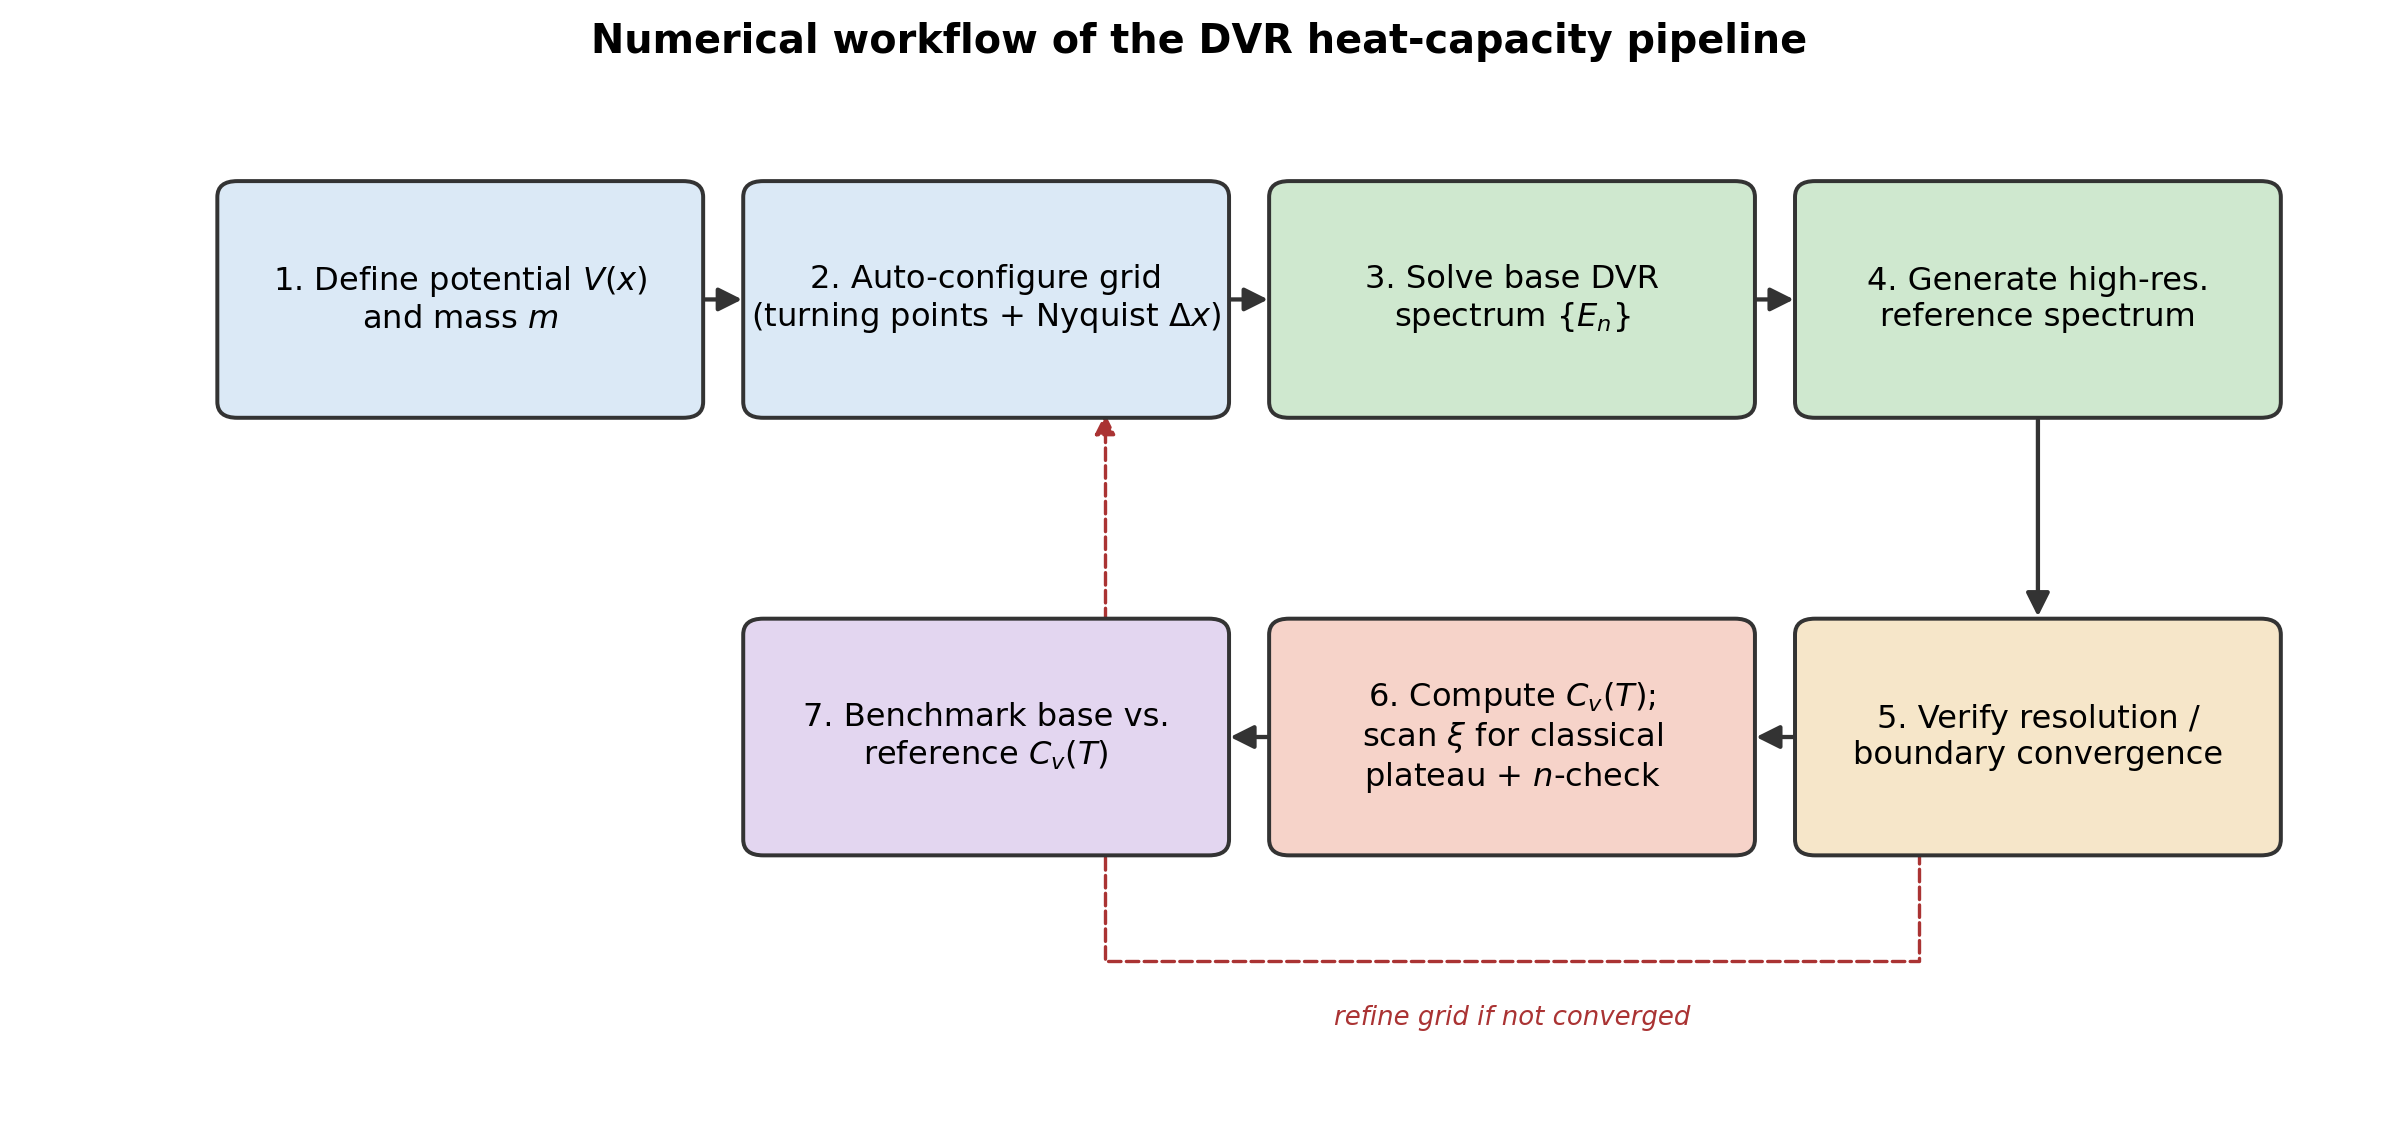
\includegraphics[draft=false,width=0.9\columnwidth]{fig_pipeline.png}
\caption{Numerical workflow of the pipeline: solve the base spectrum, generate a higher-resolution reference spectrum, verify resolution/boundary convergence against it, compute quantum $C_v(T)$ and locate the classical plateau via the $\xi/n$-scan, and benchmark base- against reference-grid $C_v(T)$. The dashed feedback path indicates that the grid is refined automatically if the convergence check of Section~\ref{sec:dvr}-D fails.}
\label{fig:pipeline}
\end{figure}

% ===================== IV. ARCHITECTURE =====================
\section{Computational Workflow}
\label{sec:arch}

The above physics is realized as a short chain of independent, system-agnostic stages (Fig.~\ref{fig:pipeline}): a grid-configuration and DVR-solve stage; a higher-resolution reference solve used as numerical ground truth for any potential (replacing the analytical HO formula once a system has no closed form); the resolution/boundary convergence check of Section~\ref{sec:dvr}; the $\xi/n$-convergence scan of Section~\ref{sec:xiconv}; and a final benchmark comparing base- and reference-grid $C_v(T)$. Because every stage after the grid configuration is written in terms of a generic energy array rather than a specific potential, switching to a new system requires changing only the potential function itself -- every other stage, including the ground-truth reference, regenerates automatically.

Table~\ref{tab:params} lists the numerical control parameters governing the $\xi$/$n$-scan and the temperature sweep, using the notation introduced in Section~\ref{sec:xiconv}. These are the settings the pipeline is presently configured with -- the same values under which the double well of Section~\ref{sec:systems}-B is now being run; several of them (notably $\text{mult}$) were tightened over the course of the semester specifically to handle the double well's narrower plateau window (Section~\ref{sec:history}), so they are not necessarily identical to the settings in force when the earlier HO benchmark of Section~\ref{sec:results} was generated.

\begin{table}[!t]
\centering
\caption{Numerical Control Parameters of the $\xi$/$n$-Scan (Current Pipeline Configuration)}
\label{tab:params}
\footnotesize
\begin{tabular}{@{}>{$}l<{$}>{\raggedright\arraybackslash}p{1.5cm}>{\raggedright\arraybackslash}p{4.35cm}@{}}
\toprule
\textbf{Symbol} & \textbf{Value} & \textbf{Role} \\
\midrule
N_{\text{lev}} & 500 & levels computed per spectrum \\
\beta_{\min},\beta_{\max} & 0.01,\ 50.0 & temperature sweep range \\
\xi_0 & 3.0 & first $\xi$-scan probe \\
\text{mult} & 1.1 & geometric step per $\xi$ iteration \\
\varepsilon_\xi & $5\times10^{-3}$ & plateau-detection tolerance, Eq.~\eqref{eq:plateautest} \\
\varepsilon_n & $10^{-4}$ & $n$-convergence tolerance, Eq.~\eqref{eq:ntest} \\
\varepsilon_{\text{DVR}} & $10^{-6}$ & resolution/boundary tolerance (Sec.~\ref{sec:dvr}-D) \\
\bottomrule
\end{tabular}
\end{table}

% ===================== V. XI/N CONVERGENCE =====================
\section{Locating the Classical Plateau}
\label{sec:xiconv}

Two nested scans turn the window of Eq.~\eqref{eq:xiwindow} into an operational procedure.

\subsection{Scanning $\xi$}
Starting from a probe value $\xi_0$, $\xi$ is stepped up geometrically and $C_v(\xi)$ is recomputed at each step from the scaled spectrum $E_n\to E_n/\xi^2$. Two outcomes are distinguished: a run of near-constant $C_v$ values, accepted as the plateau of Eq.~\eqref{eq:xiwindow}, versus a sudden drop toward zero, which signals that $\xi$ has entered the finite-$N$ regime of Eq.~\eqref{eq:xiupper} rather than the physical classical limit. This second outcome is not a failure of the physics -- it is exactly the Schottky-type collapse discussed in Section~\ref{sec:schottky}, and distinguishing it from a genuine plateau is the entire point of the scan (see Fig.~\ref{fig:xi_convergence} for a worked example).

\smallskip
\noindent\textbf{Input:} spectrum $\{E_n\}$, $\beta$, probe $\xi_0$, tolerance $\varepsilon_\xi$. \quad
\textbf{Output:} converged scaling factor $\xi_{\text{conv}}$ and classical-limit heat capacity $C_v^{\text{conv}}$, or a reported failure if no plateau is found before collapse.
\begin{equation}
\text{(plateau test)}\qquad \big|C_v(\xi)-C_v(\xi/\text{mult})\big| < \varepsilon_\xi .
\label{eq:plateautest}
\end{equation}

\subsection{Checking How Many Levels Were Actually Needed}
A second, independent scan asks how many of the computed levels were actually required to reach that plateau: $C_v$ is recomputed at $\xi_{\text{conv}}$ using only the lowest $n$ levels, for increasing $n$, until it stops changing (Fig.~\ref{fig:n_convergence}). A converged answer using only a handful of low-lying levels indicates a robust, physically meaningful result, whereas one that only stabilizes near the very top of the computed spectrum is a warning sign that the truncation itself, not genuine physics, is shaping the curve (Section~\ref{sec:schottky}).

\smallskip
\noindent\textbf{Input:} spectrum $\{E_n\}$, $\beta$, $\xi_{\text{conv}}$, tolerance $\varepsilon_n$. \quad
\textbf{Output:} minimal level count $n_{\text{conv}}$ needed for a converged $C_v$.
\begin{equation}
\text{($n$-convergence test)}\qquad \big|C_v(n{+}1)-C_v(n)\big| < \varepsilon_n .
\label{eq:ntest}
\end{equation}

% ===================== VI. SYSTEMS =====================
\section{Systems Studied}
\label{sec:systems}

\subsection{Harmonic Oscillator -- Validation Case}
The HO is the reference system used to validate the numerical method against Eq.~\eqref{eq:cvho} before trusting the same pipeline on systems with no closed-form answer. Figures~\ref{fig:ho_energy_comparison}--\ref{fig:n_convergence} show the full set of validation diagnostics produced so far, all for $N_{\text{lev}}=500$.

\begin{figure}[!t]
\centering
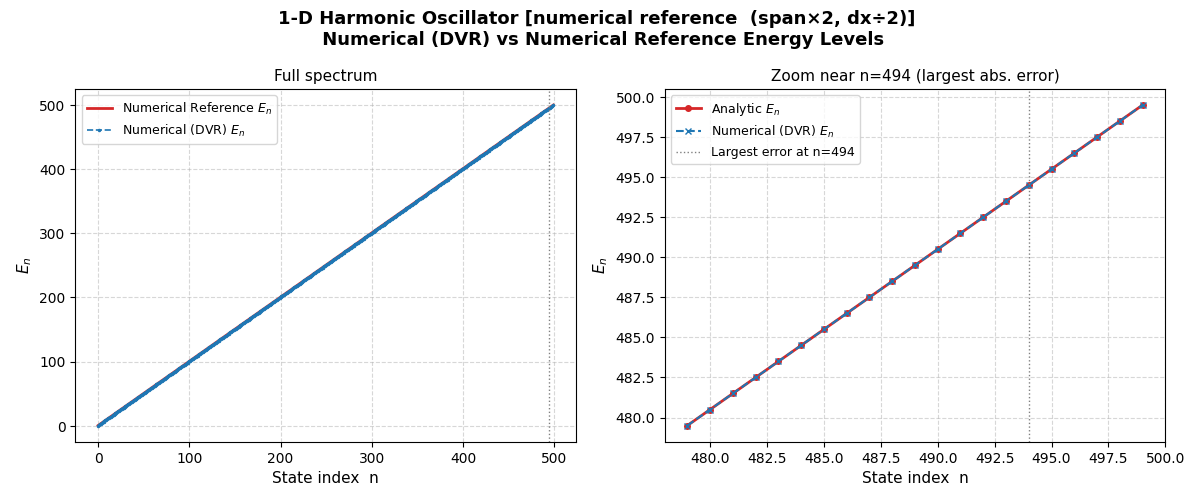
\includegraphics[draft=false,width=0.9\columnwidth]{fig_ho_energy_comparison.png}
\caption{Base-grid vs. numerical-reference energy levels $E_n$ for the HO, full spectrum (left) and zoomed to the ten states around the largest absolute error, near $n=494$ (right). The two are visually indistinguishable at either scale.}
\label{fig:ho_energy_comparison}
\end{figure}

\begin{figure}[!t]
\centering
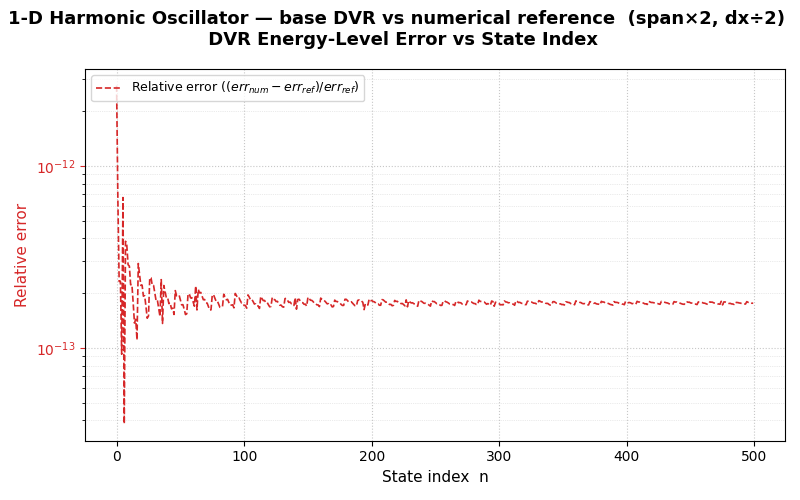
\includegraphics[draft=false,width=0.9\columnwidth]{fig_ho_error_vs_n.png}
\caption{Relative error between base-grid and reference-grid energy levels vs. state index $n$. The error is already at the $10^{-13}$--$10^{-12}$ level for the very lowest states and settles to a flat $\sim\!1.5\times10^{-13}$ plateau by $n\approx100$ -- consistent with both grids being converged to machine precision, so that only floating-point round-off remains.}
\label{fig:ho_error_vs_n}
\end{figure}

\begin{figure}[!t]
\centering
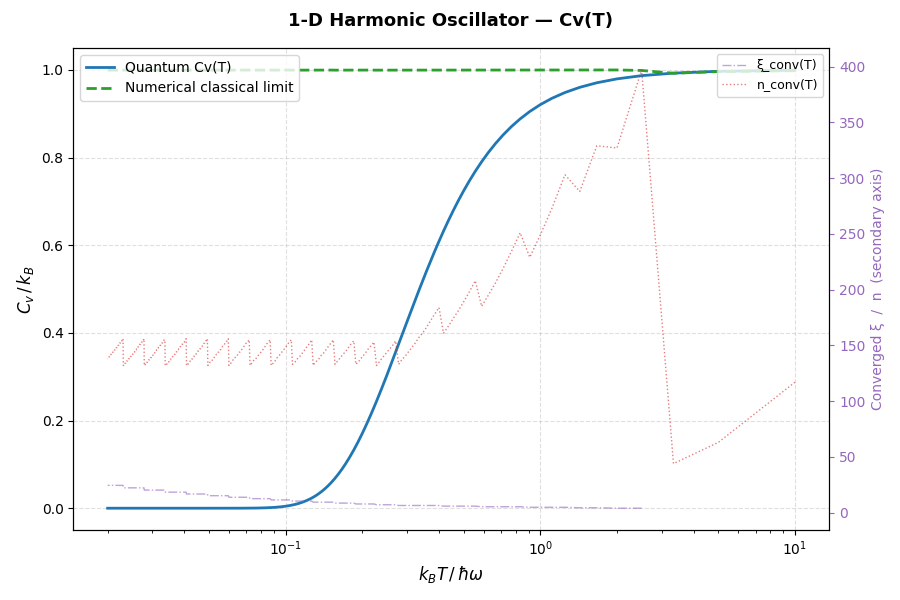
\includegraphics[draft=false,width=0.9\columnwidth]{fig_cv_summary_ho.png}
\caption{Quantum $C_v(T)$ (solid) and numerical classical limit (dashed) for the HO, together with the converged $\xi_{\text{conv}}(T)$ and $n_{\text{conv}}(T)$ on the secondary axis. The classical limit tracks $C_v/k_B=1$ across the full range where the $\xi$-scan converges; $n_{\text{conv}}$ rises with $T$ as more levels are needed to represent a hotter thermal state.}
\label{fig:cv_summary_ho}
\end{figure}

\begin{figure}[!t]
\centering
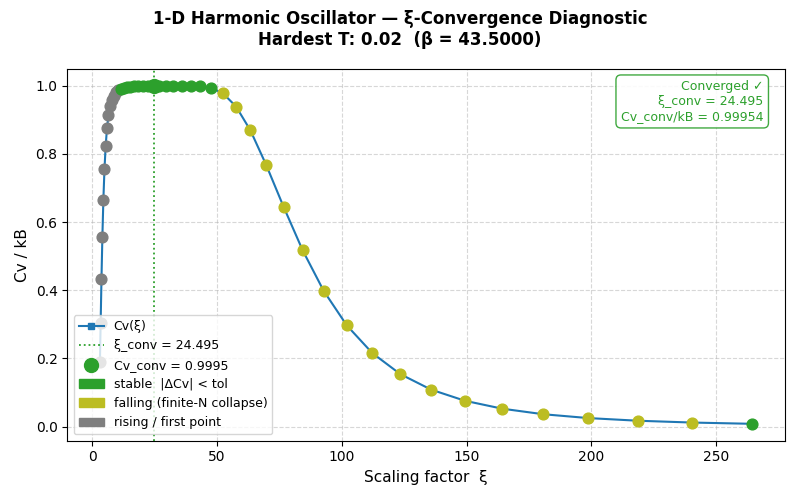
\includegraphics[draft=false,width=0.9\columnwidth]{fig_xi_convergence.png}
\caption{$\xi$-convergence diagnostic at the hardest (lowest) temperature in the sweep, $k_BT/\hbar\omega=0.02$. $C_v(\xi)$ rises (grey), stabilizes onto the plateau (green, $\xi_{\text{conv}}=24.5$, $C_v^{\text{conv}}/k_B=0.9995$), and eventually collapses (yellow) once $\xi$ pushes the scaled spectrum into the finite-$N$ regime of Eq.~\eqref{eq:xiupper} -- the numerical Schottky-type failure mode of Section~\ref{sec:schottky}.}
\label{fig:xi_convergence}
\end{figure}

\begin{figure}[!t]
\centering
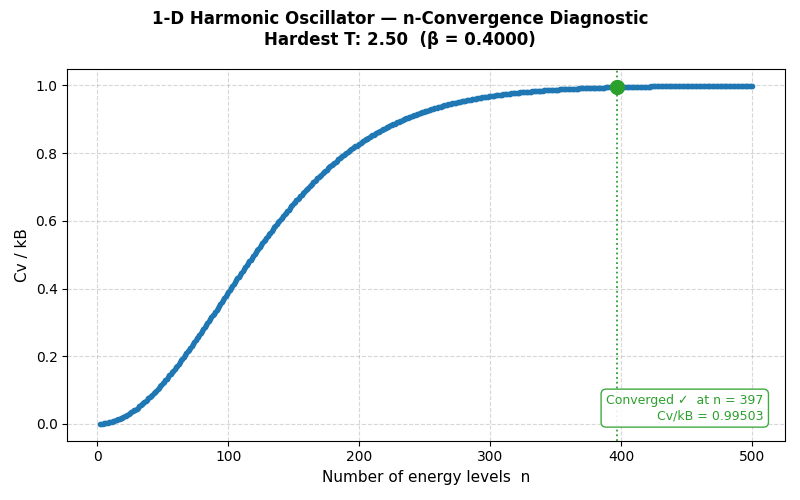
\includegraphics[draft=false,width=0.9\columnwidth]{fig_n_convergence.png}
\caption{$n$-convergence diagnostic at the hardest temperature in the sweep, $k_BT/\hbar\omega=2.50$. $C_v(n)$ rises smoothly and is converged (to within $\varepsilon_n$) at $n_{\text{conv}}=397$ out of the 500 computed levels, with $C_v/k_B=0.995$ at that point.}
\label{fig:n_convergence}
\end{figure}

\subsection{Symmetric / Asymmetric Double Well -- Current System}
The potential currently under study is the quartic double well
\begin{equation}
V(x) = \frac14 x^4 + b\,x^3 - \frac12 x^2,
\label{eq:doublewell}
\end{equation}
with $b=-0.5$ in the active run; setting $b=0$ recovers the purely symmetric double well. The $b\neq0$ term probes the asymmetric case discussed with the supervisor (Meeting~8): comparing the near-well region of a deep asymmetric well against the symmetric HO result as an additional sanity check. This is the first anharmonic potential in the pipeline, and it is a meaningfully harder test than the HO: its levels scale as $E_n\propto n^{4/3}$ rather than linearly, so the level spacing $\Delta E(E)$ shrinks with energy far more slowly, which narrows the plateau window of Eq.~\eqref{eq:xiwindow} (Section~\ref{sec:history}). Numerical results for this potential are still being produced and are not yet included in this report (Section~\ref{sec:future}).

The double well also has a genuine two-scale spectrum: a finite central barrier supports a near-degenerate pair of levels below the barrier, split by quantum tunnelling, separated by a much larger gap from the states above it. In the WKB approximation, the size of this splitting is exponentially small in the barrier's classical action,
\begin{equation}
\Delta_{\text{tunnel}} \sim \hbar\omega_0\,\exp\!\left(-\frac{1}{\hbar}\int_{-a}^{a}\!\sqrt{2m\big(V(x)-E_0\big)}\;dx\right),
\label{eq:wkbsplitting}
\end{equation}
where $\pm a$ are the inner classical turning points at the ground-state energy $E_0$ of a single well. Equation~\eqref{eq:wkbsplitting} is the physical origin of the Schottky discussion in Section~\ref{sec:schottky}: it sets the temperature scale, $k_BT_{\text{peak}}\sim\Delta_{\text{tunnel}}$, at which a genuine low-temperature feature in $C_v(T)$ -- and a candidate quantum-over-classical enhancement of the kind motivating this project (Section~\ref{sec:intro}) -- is expected.

% ===================== VII. SCHOTTKY =====================
\section{The Schottky Anomaly and Its Relevance to This Project}
\label{sec:schottky}

A Schottky anomaly is a peak in $C_v(T)$ characteristic of systems with a small, effectively finite number of accessible energy levels: at low $T$ only the ground state is populated ($C_v\to0$), $C_v$ rises to a maximum once $k_BT$ becomes comparable to the level spacing, and then falls again as the available levels saturate and further heating produces little additional entropy change \cite{gelbwaser2018,kozin2025}. It is ``anomalous'' precisely because $C_v$ for a system with an effectively infinite, evenly-filling ladder of states (like the HO in its classical limit) does not fall back down -- it saturates at the equipartition value instead.

The unifying idea behind both roles this feature plays in the project is that $C_v(T)$, as built from Eq.~\eqref{eq:cv_general}, is mathematically blind to \emph{why} a spectrum has a top rung -- it only responds to the fact that one exists. A hard edge in the level ladder produces the same qualitative peak-and-decay signature whether that edge is a fundamental energy gap or an artifact of a finite numerical basis.

\subsection{Schottky Collapse as a Numerical Artifact}
Any DVR calculation truncates the spectrum at a finite $N_{\text{lev}}$. Once $k_BT$ (or, equivalently, the scaled thermal scale under $\xi$) approaches the energy of the \emph{highest computed level}, that finite basis behaves exactly like a small-level-count Schottky system: $C_v$ turns over and collapses toward zero, even though the true, infinite-level system's $C_v$ would continue rising toward the classical plateau. This is precisely the failure mode that the plateau scan of Section~\ref{sec:xiconv} is built to detect and reject (Fig.~\ref{fig:xi_convergence}), Eq.~\eqref{eq:xiupper} being its quantitative statement. In this sense every finite spectrum computed by this pipeline is a latent Schottky system, and the entire $\xi$/$n$-convergence procedure exists to keep the reported classical limit on the correct side of that artifact.

\subsection{A Genuine Schottky Signature in the Double Well}
The second connection is physical rather than numerical. The double well's tunnelling-split doublet of Eq.~\eqref{eq:wkbsplitting} is a small energy gap nested inside a much larger one (the gap to the states above the barrier) -- the textbook precondition for a genuine, physical Schottky peak, and tunnelling-split doublets in symmetric double-well potentials are indeed reported to produce narrow Schottky features in the literature \cite{kozin2025}. If confirmed numerically for Eq.~\eqref{eq:doublewell}, a low-temperature bump in $C_v(T)$ near $k_BT\sim\Delta_{\text{tunnel}}$, well before the climb to the classical plateau, would be a real thermodynamic feature of this system rather than a truncation artifact -- and would directly address the goal set in Meeting~8 of finding a potential where the quantum $C_v$ transiently exceeds the classical value. As discussed in Section~\ref{sec:intro}, this kind of enhanced energy-fluctuation regime is exactly the mechanism identified in \cite{campisifazio2016} as a route to approaching Carnot efficiency at finite power, which is the broader motivation this semester's tool is meant to serve.

Distinguishing the two cases in practice comes down to where the feature sits relative to $n_{\text{conv}}(T)$: a genuine tunnelling-doublet peak should be well converged using only the lowest handful of levels, while an artifactual collapse only ever appears once $n_{\text{conv}}$ approaches $N_{\text{lev}}$.

% ===================== VIII. RESULTS =====================
\section{Results and Validation}
\label{sec:results}

\subsection{Harmonic-Oscillator Validation}
Figure~\ref{fig:ho_error_vs_n} shows that the base and reference grids agree to within machine precision across the full computed spectrum, with a relative error plateau of $\sim\!1.5\times10^{-13}$. This propagates through to the thermodynamic observable: Fig.~\ref{fig:cv_benchmark_quantum} shows the quantum $C_v(T)$ agreeing with the reference to a maximum absolute error of $3.84\times10^{-13}\,k_B$, Fig.~\ref{fig:cv_benchmark_quantum_rel} shows the same comparison as a relative error (meaningful only away from the very lowest temperatures, where both curves numerically underflow toward zero), and Fig.~\ref{fig:cv_benchmark_classical} shows the classical-limit curve agreeing to a maximum relative error of $6.34\times10^{-14}$.

\begin{figure}[!t]
\centering
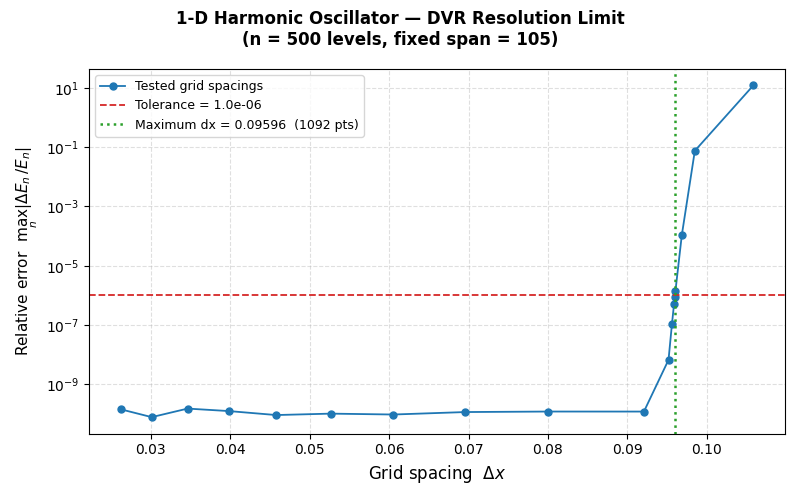
\includegraphics[draft=false,width=0.9\columnwidth]{fig_dvr_res_dx.png}
\caption{DVR resolution limit: relative eigenvalue error vs. grid spacing $\Delta x$, at fixed span (105) and 500 requested levels. Spacings up to $\Delta x\approx0.096$ (1092 points) remain below the $10^{-6}$ tolerance; the error rises by many orders of magnitude just beyond that point.}
\label{fig:dvr_res_dx}
\end{figure}

\begin{figure}[!t]
\centering
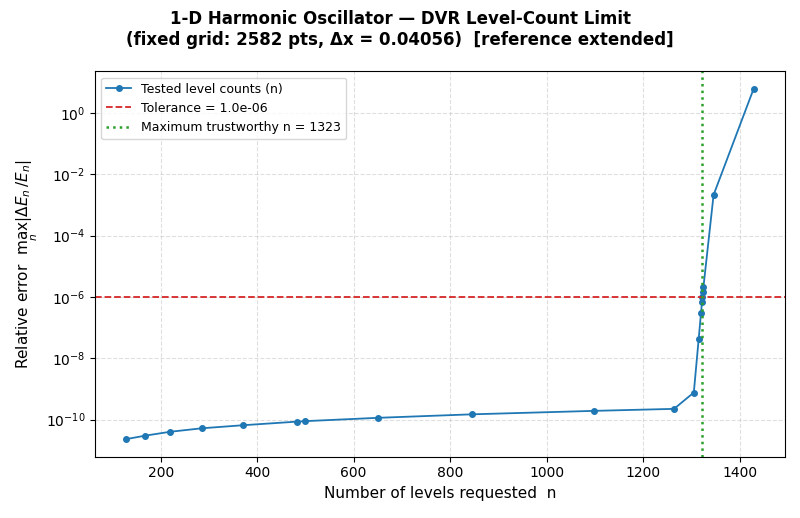
\includegraphics[draft=false,width=0.9\columnwidth]{fig_dvr_res_n.png}
\caption{DVR level-count limit: relative eigenvalue error vs. requested level count $n$, at a fixed grid (2582 points, $\Delta x=0.04056$). The maximum trustworthy count is $n=1323$, i.e. $1323/2582\approx0.51$ of the grid's points -- a direct confirmation of the rule of thumb that only roughly the lower half of a DVR spectrum should be trusted, since the highest-index states are the first whose local momentum exceeds what the fixed spacing can resolve.}
\label{fig:dvr_res_n}
\end{figure}

\begin{figure}[!t]
\centering
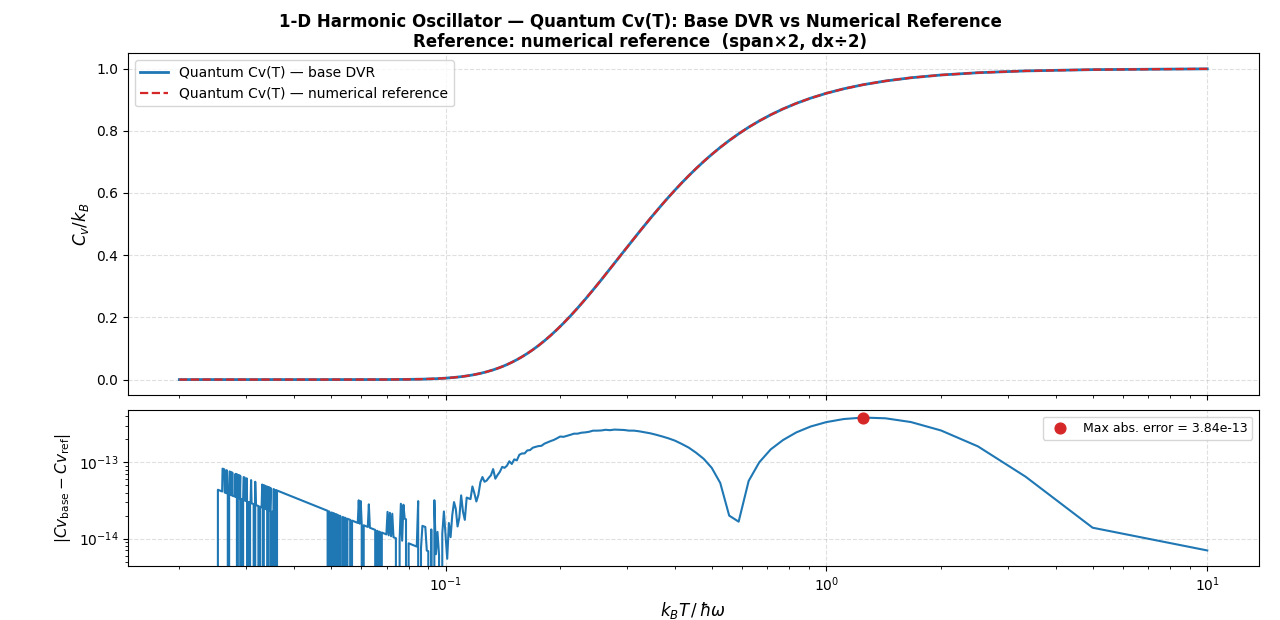
\includegraphics[draft=false,width=0.9\columnwidth]{fig_cv_benchmark_quantum_abs.png}
\caption{Quantum $C_v(T)$: base grid vs. numerical reference, with the absolute error shown below. Maximum absolute error $3.84\times10^{-13}\,k_B$.}
\label{fig:cv_benchmark_quantum}
\end{figure}

\begin{figure}[!t]
\centering
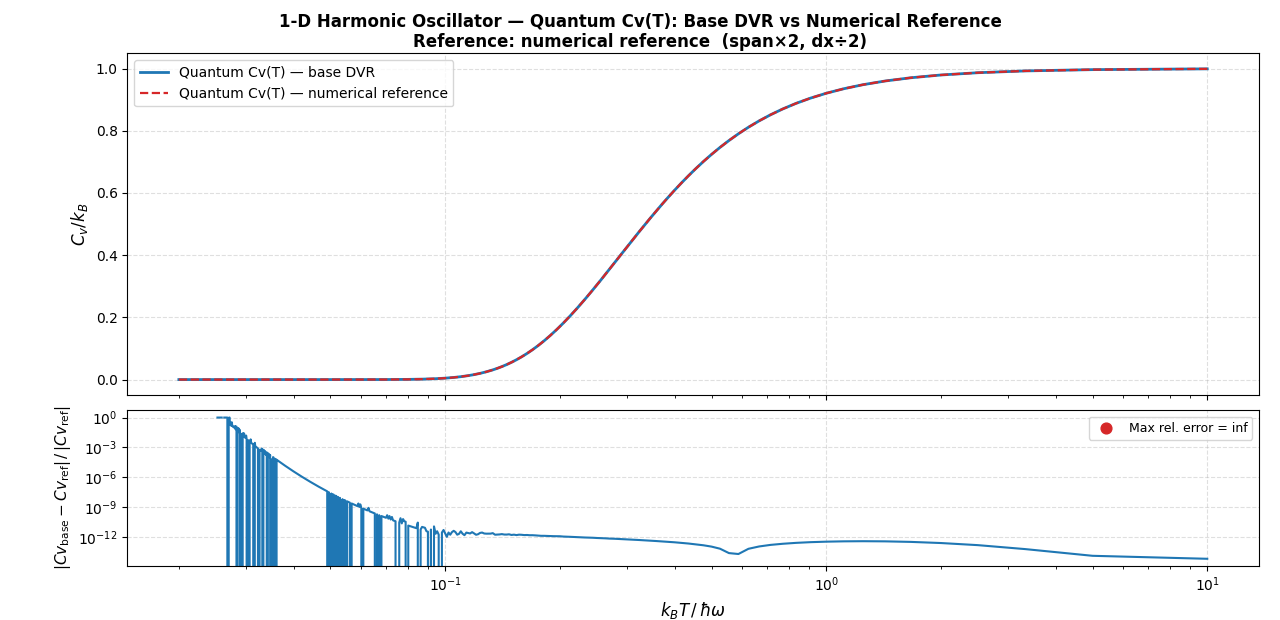
\includegraphics[draft=false,width=0.9\columnwidth]{fig_cv_benchmark_quantum_rel.png}
\caption{Same comparison as Fig.~\ref{fig:cv_benchmark_quantum}, shown as a relative rather than absolute error. The spikes at the lowest temperatures are a numerical artifact, not a real loss of accuracy: both $C_v^{\text{base}}$ and $C_v^{\text{ref}}$ underflow toward zero there, so their already-tiny absolute difference is being divided by an equally tiny reference value. This is why the reported maximum relative error is formally infinite, while Fig.~\ref{fig:cv_benchmark_quantum} shows the same comparison is in fact accurate to $10^{-13}\,k_B$ throughout.}
\label{fig:cv_benchmark_quantum_rel}
\end{figure}

\begin{figure}[!t]
\centering
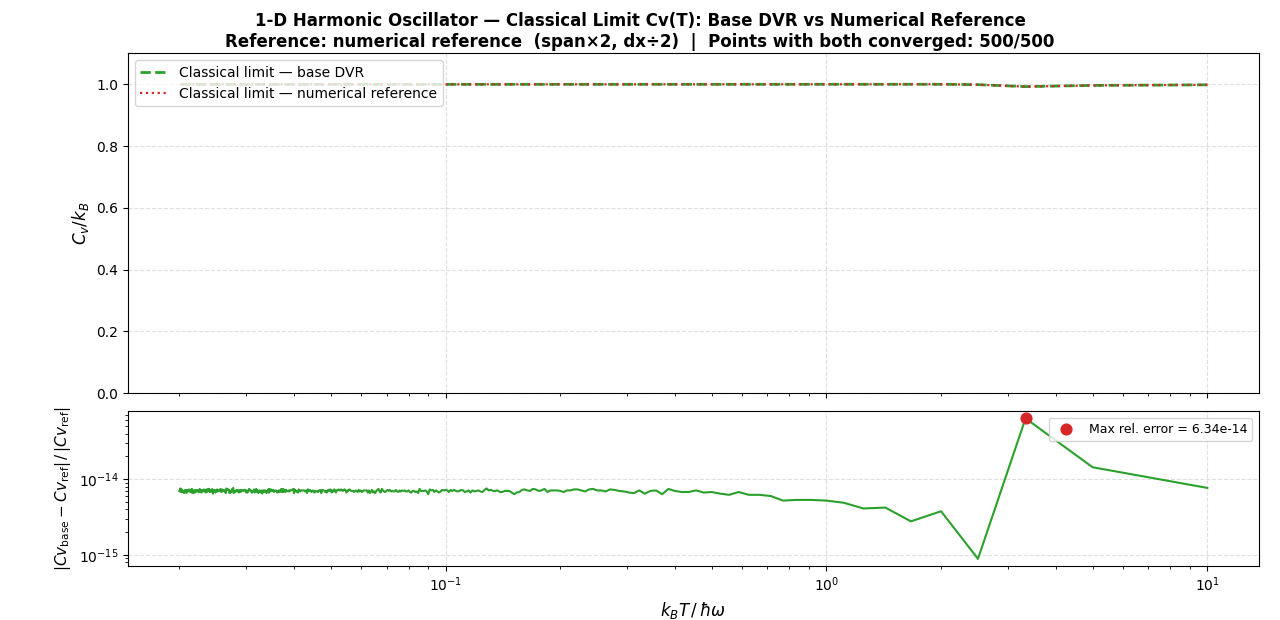
\includegraphics[draft=false,width=0.9\columnwidth]{fig_cv_benchmark_classical.png}
\caption{Classical-limit $C_v(T)$: base grid vs. numerical reference, with the relative error shown below. All 500 temperature points converged on both grids; maximum relative error $6.34\times10^{-14}$.}
\label{fig:cv_benchmark_classical}
\end{figure}

\subsection{Double-Well Progress}
The double well of Eq.~\eqref{eq:doublewell} is now running end-to-end through the same workflow used for the HO, with no changes beyond the potential definition itself -- direct evidence that the system-agnostic design of Section~\ref{sec:arch} succeeded in its goal. Quantitative results for this system, and in particular whether the low-temperature feature predicted by Eq.~\eqref{eq:wkbsplitting} is visible, are the main outstanding deliverable for the summer continuation described in Section~\ref{sec:future}.

% ===================== IX. VERSION HISTORY =====================
\section{Numerical Refinements This Semester}
\label{sec:history}

Table~\ref{tab:refinements} summarizes the main numerical issues encountered and resolved this semester, all of which trace back to the physical reasoning of Sections~\ref{sec:theory}--\ref{sec:xiconv}.

\begin{table}[!t]
\centering
\footnotesize
\caption{Key Numerical Refinements and Their Physical Motivation}
\label{tab:refinements}
\begin{tabular}{@{}>{\raggedright\arraybackslash}p{2.55cm}>{\raggedright\arraybackslash}p{5.15cm}@{}}
\toprule
\textbf{Issue} & \textbf{Resolution and motivation} \\
\midrule
Manual grid tuning & Replaced by the local Nyquist criterion of Section~\ref{sec:dvr}-C, removing guesswork for new potentials. \\
Insufficient tail padding for anharmonic wells & Fixed span padding under-estimated wavefunction tails for quartic/double-well potentials; replaced with iterative widening until eigenvalues stop changing (Section~\ref{sec:dvr}-C). \\
Narrow plateau window for anharmonic spectra & Because $E_n\propto n^{4/3}$ in the double well, Eq.~\eqref{eq:xiwindow} narrows relative to the HO's linear spectrum; the $\xi$-step was made more granular so the scan reliably lands inside the window before finite-$N$ collapse. \\
Aliasing at hard-wall potentials & Restricted the DVR core to smooth potentials only (Section~\ref{sec:dvr}-B), since discontinuities are not band-limited and cannot be represented on any finite grid. \\
\bottomrule
\end{tabular}
\end{table}

% ===================== X. FUTURE WORK =====================
\section{Future Work}
\label{sec:future}

Two structural changes are planned for the summer continuation of this project.

\subsubsection{FFT-accelerated matrix-free diagonalization}
The current solver builds a dense $N\times N$ Hamiltonian and diagonalizes it directly, which scales as $\mathcal{O}(N^3)$ in time and $\mathcal{O}(N^2)$ in memory -- the main obstacle to pushing $N_{\text{lev}}$ higher for anharmonic systems. Because the kinetic operator is diagonal in momentum space, its action on a wavefunction can instead be applied via a Fourier transform at a cost of $\mathcal{O}(N\log N)$ per application rather than $\mathcal{O}(N^2)$ for an explicit matrix multiply. Combined with an iterative (Krylov-subspace) eigensolver that needs only a modest number of such applications per eigenvalue, this removes the dense-matrix memory bottleneck entirely and should enable thousands of levels where hundreds are currently the practical ceiling.

\subsubsection{Adaptive spatial grid mapping}
The uniform sinc-DVR grid is inefficient for potentials whose wavefunctions oscillate rapidly near the well bottom and decay slowly in the tails: the fixed spacing must satisfy the Nyquist criterion at the point of \emph{highest} local momentum, oversampling everywhere else. An analytical coordinate map from a uniform computational coordinate rescales the local grid spacing, compressing points where the local de Broglie wavelength is short and stretching them in the classically forbidden tails. Satisfying the Nyquist criterion locally rather than globally is expected to reduce the required grid points by a factor of $3$--$4$.

Beyond these two structural changes, the immediate next steps are to (i) complete and quantitatively characterize the double-well run of Section~\ref{sec:systems}, including the symmetric-vs-asymmetric comparison from Meeting~8, and produce the corresponding figures (potential shape, $C_v(T)$ summary) using the same plotting tools now in place for the HO; (ii) test the WKB prediction of Eq.~\eqref{eq:wkbsplitting} against the low-$T$ behavior of the numerical $C_v(T)$, using the $n_{\text{conv}}$ diagnostic to rule out a truncation artifact; (iii) validate the double-well pipeline against its own harmonic limit, as proposed in Meeting~3: continuously reduce the quartic and cubic terms of Eq.~\eqref{eq:doublewell} toward zero and confirm that the computed spectrum and $C_v(T)$ converge smoothly onto the HO benchmark of Section~\ref{sec:results}, giving an internal consistency check that is independent of the WKB estimate; (iv) compare the resulting $C_v(T)$ against literature values for comparable model potentials, as discussed in Meeting~8, to cross-check the pipeline against results obtained by other methods; and (v), motivated by Section~\ref{sec:intro}, begin systematically scanning across potentials for temperature windows where quantum $C_v$ exceeds classical $C_v$, as a first step toward the project's longer-term heat-machine question.

% ===================== XI. CONCLUSION =====================
\section{Conclusion}

This semester's work built the numerical groundwork for a longer-term search for quantum-enhanced heat machine performance: a general-purpose pipeline that computes $C_v(T)$, and its classical counterpart, for any smooth one-dimensional potential. Every design choice in that pipeline -- the sinc-DVR's Nyquist-limited grid, the restriction to smooth potentials, and the $\xi$-scaling as a controlled version of $\hbar\to0$ -- follows from the same semiclassical reasoning connecting discrete spectra to their classical continuum limit. The harmonic-oscillator benchmark confirms the method reproduces the exact analytical result to within machine precision, and the same pipeline is now running, unmodified, on the anharmonic double well. The Schottky-anomaly discussion of Section~\ref{sec:schottky} highlights why this validation effort matters beyond the HO case: distinguishing a genuine quantum enhancement of $C_v$ from a numerical truncation artifact is exactly the distinction this project's longer-term goal depends on, and it is precisely what the convergence machinery built this semester is designed to do.

\section*{Code Availability}
The full source code, module-level documentation, figures, and reference literature cited in this report are maintained at:\\
\url{https://github.com/NadavJ180/Research-Project}

% ===================== REFERENCES =====================
\begin{thebibliography}{9}

\bibitem{gelbwaser2018}
D. Gelbwaser-Klimovsky, A. Bylinskii, D. Gangloff, R. Islam, A. Aspuru-Guzik, and V. Vuletic, ``Single-atom heat machines enabled by energy quantization,'' \emph{Phys. Rev. Lett.}, vol. 120, p. 170601, Apr. 2018.

\bibitem{colbertmiller1992}
D. T. Colbert and W. H. Miller, ``A novel discrete variable representation for quantum mechanical reactive scattering via the S-matrix Kohn method,'' \emph{J. Chem. Phys.}, vol. 96, no. 3, pp. 1982--1991, 1992.

\bibitem{lightcarrington2000}
J. C. Light and T. Carrington Jr., ``Discrete-variable representations and their utilization,'' in \emph{Advances in Chemical Physics}, vol. 114. Hoboken, NJ: John Wiley \& Sons, 2000, pp. 263--310.

\bibitem{campisifazio2016}
M. Campisi and R. Fazio, ``The power of a critical heat engine,'' \emph{Nat. Commun.}, vol. 7, p. 11895, 2016.

\bibitem{ye2017}
Z. Ye, Y. Hu, J. He, and J. Wang, ``Universality of maximum-work efficiency of a cyclic heat engine based on a finite system of ultracold atoms,'' \emph{Sci. Rep.}, vol. 7, p. 6289, 2017.

\bibitem{kozin2025}
V. K. Kozin, D. Miserev, D. Loss, and J. Klinovaja, ``Schottky anomaly in a cavity-coupled double quantum well,'' \emph{Phys. Rev. Res.}, vol. 7, p. 033239, 2025.

\end{thebibliography}

\end{document}